\documentclass[12pt]{article}
\usepackage{amsmath}
\usepackage{latexsym}
\usepackage{amsfonts}
\usepackage{amssymb}
\usepackage{graphicx}
\usepackage{txfonts}
\usepackage{wasysym}
\usepackage{adjustbox}
\usepackage{ragged2e}
\usepackage{tabularx}
\usepackage{hhline}
\usepackage{float}
\usepackage{multirow}
\usepackage{makecell}
\usepackage{fancyhdr}
\usepackage[utf8]{inputenc}
\usepackage[T1]{fontenc}
\usepackage[a4paper,bindingoffset=0.2in,headsep=0.5cm,left=1in,right=1in,bottom=3cm,top=2cm,headheight=2cm]{geometry}
\usepackage{hyperref}
\usepackage{listings}
\usepackage[most]{tcolorbox}

\lstset{language=C,basicstyle=\scriptsize\ttfamily,keywordstyle=\bfseries, commentstyle=\textit,stringstyle=\ttfamily, showspaces=false,showstringspaces=false, frame=single,
  breaklines=true,
  postbreak=\mbox{\textcolor{red}{$\hookrightarrow$}\space},
}

\everymath{\displaystyle}
\pagestyle{fancy}
\fancyhf{}
\rfoot{Page \thepage}
\begin{document}
\sloppy 

\begin{center}


\includegraphics[width=0.2\textwidth]{fig/logotpt}
\vspace{10 pt}\\
\Huge TTool \\
\vspace{10 pt}
\Large \url{ttool.telecom-paristech.fr}
\vspace{20 pt}\\
\underline{\Large SysML-Sec Tutorial}
\vspace{30 pt}
\end{center}

\begin{table}[H]
\large
\centering
\begin{adjustbox}{width=\textwidth}
\begin{tabular}{ |p{1.6cm}|p{6.0cm}|p{4.2cm}|p{4.2cm}| }
\hhline{----}
 & \textbf{Document Manager} & \textbf{Contributors}  & \textbf{Checked by}  \\ 
\hhline{----}
\textbf{Name}   & Ludovic APVRILLE & \multirow{2}{*}{Ludovic APVRILLE} &
\multirow{2}{*}{Ludovic APVRILLE} \\
\hhline{--~~}
\textbf{Contact} & ludovic.apvrille@telecom-paristech.fr &  &  \\ 
\hhline{--~~}
\textbf{Date} & \today &  &  \\ 
\hline
\end{tabular}
\end{adjustbox}
\end{table}

\newpage
\tableofcontents

% \newpage
% \listoffigures

\newpage
\section{Preface}

\subsection{Table of Versions}

\begin{table}[H]
\large
\centering
\begin{adjustbox}{width=\textwidth}
\begin{tabular}{ |p{1.5cm}|p{2.5cm}|p{9.0cm}|p{3.0cm}| }
\hhline{----}
\textbf{Version} & \textbf{Date} & \textbf{Description  $  \&  $  Rationale of
Modifications} & \textbf{Sections Modified} \\
\hhline{----}
1.0 & April 3rd, 2018 & First draft &  \\ 
\hline
\end{tabular}
\end{adjustbox}
\end{table}

\subsection{Table of References and Applicable Documents}

\begin{table}[H]
\large
\centering
\begin{adjustbox}{width=\textwidth}
\begin{tabular}{ |p{2.66in}|p{2.66in}|p{0.95in}|p{0.43in}| }
\hhline{----}
\textbf{Reference} & \textbf{Title  $  \&  $  Edition} & \textbf{Author or
Editor} & \textbf{Year}
\\
\hhline{----}
 &  &  &  \\ 
\hline
\end{tabular}
\end{adjustbox}
\end{table}

\subsection{Acronyms and glossary}

\begin{table}[H]
\large
\centering
\begin{adjustbox}{width=\textwidth}
\begin{tabular}{ |p{1.24in}|p{5.45in}| }
\hhline{--}
\textbf{Term} & \textbf{Description} \\ 
\hhline{--}
 &  \\ 
\hline
\end{tabular}
\end{adjustbox}
\end{table}

\subsection{Summary}

This document describes how to use SysML-Sec using simple examples\footnote{This document has been started in the scope of the AQUAS european project}. In particular, it covers requirements, attack trees, HW/SW partitioning and software design.

\newpage

\section{Configuration}\label{sec:conf}
\subsection{TTool configuration}
At first, if not already configured\footnote{Your version of TTool should be already configured}, you must open the configuration file of TTool. The default file is located in:
\begin{verbatim}
TTool/bin/config.xml
\end{verbatim}
Open your configuration file, and add the following lines accordingly with your TTool and ProVerif installation:
\begin{itemize}
\item Directory in which formal specifications for security proofs are generated:
\begin{verbatim}
<ProVerifCodeDirectory data="../proverif/" />
\end{verbatim}
\item Path to the proverif executable file:
\begin{verbatim}
<ProVerifVerifierPath data="/opt/proverif/proverif" />
\end{verbatim}
\item Host on which the proof will be started (for example, you could execute this proof on a dedicated machine if the "ProVerifCodeDirectory" is reachable from that dedicated machine):
\begin{verbatim}
<ProVerifVerifierHost data="localhost" />
\end{verbatim}
\end{itemize}


\subsection{External tools}
The  configuration for the DIPLODOCUS simulator assumes that a \textbf{C compiler}, referenced by the provided Makefile (default = "gcc"\footnote{\url{https://gcc.gnu.org/}}) is installed on your machine, as well as the \textbf{POSIX-1 librairies}. Also, a Makefile utility must be installed (e.g., "GNU make"\footnote{\url{https://www.gnu.org/software/make/}}).

\newpage
\section{Getting started with a toy example}\label{sec:example}
This very first example explains how to use the main capabilities of SysML-Sec.

\subsection{Getting the example}
Be sure to get the latest version of TTool including the remote loading of models (March 2018 and after). Do: File, Open from TTool repository, and select "SysMLSecTutorial.xml".

\subsection{Understanding the model}
The first tab of the model presents an overview of the SysML-Sec methodology (see Figure \ref{fig:method}). Each stage of the method is represented with a rectangle that contains a link to the corresponding diagrams.  All other tabs correspond to the diagrams of the model.


\begin{figure*}[htbp]
\centering
\includegraphics[width=0.99\textwidth]{build/method-svg.pdf}

\caption{The first diagram represents the SysML-Sec method. Each stage of the method is represented by a rectangle that contains a link to all diagrams of the corresponding stage.} \label{fig:method}
\end{figure*}

\subsection{Security requirements}
Security requirements are captured with a SysML requirement diagram that is extended in the following ways:
\begin{enumerate}
\item Requirements can be tagged as "Functional", "Non Functional", "Privacy", "Confidentiality", "Non Repudiation", "Controlled Access", "Availability", "Immunity", "Data Origin Authenticity", "Freshness", "Business", "Stakeholder Need", "Other"
\item Requirements have a \textbf{risk} attribute (low, medium, high).
\item References to other diagram elements can be added and linked to requirements with a "satisfy" relation. "elt satifies req" means that elt is part of the mechanisms used to satisfy the referenced requirement.
\end{enumerate}

The requirement diagram of Figure \ref{fig:req1} shows a confidentiality requirements that states that all functional communication paths should be confidential.

\begin{figure*}[htbp]
\centering
\includegraphics[width=0.5\textwidth]{build/requirements1-svg.pdf}
\caption{Security requirements (version \#1)} \label{fig:req1}
\end{figure*}

\subsection{Functional Model (version 1)}
The functional model is built upon the merge of a  SysML Block Definition Diagram and a SysML Internal Block Diagram, see Figure \ref{fig:fv1}. The functional view contains two blocks : T1 and T2.  The functional behavior of T1 and T2 is captured with Activity diagrams, as displayed on the left and right of Figure \ref{fig:fv1}. Basically, T1 writes one data sample, and T2 reads one data sample.


\begin{figure*}[htbp]
\centering
\includegraphics[width=0.1\textwidth]{build/fv1_t1-svg.pdf}
\includegraphics[width=0.7\textwidth]{build/fv1-svg.pdf}
\includegraphics[width=0.1\textwidth]{build/fv1_t2-svg.pdf}
\caption{Functional View (version \#1)} \label{fig:fv1}
\end{figure*}

As shown on the block diagram, T1 and T2 are connected with a data communication channel. Since this communication channel must be secure (see Figure \ref{fig:req1}), we can now enrich the Requirement Diagram with a new security requirement connected to the initial security requirement (see Figure \ref{fig:req2})

\begin{figure*}[htbp]
\centering
\includegraphics[width=0.5\textwidth]{build/requirements2-svg.pdf}
\caption{Security requirements (version \#2)} \label{fig:req2}
\end{figure*}

We also enrich the communication channel $comm$ between T1 and T2 with a confidentiality property, as shown by the \textit{grey lock} with the question marks just next to the port of comm in T1 (Figure \ref{fig:fv1}).

\subsection{Architecture and Mapping Models (version 1)}

A simple architecture model and mapping is shown in Figure \ref{fig:mapping1}. T1 and T2 are mapped on CPU1 and CPU2, respectively. The channel between T1 and T2 is mapped on "MainBus" and on "MainMemory".

\begin{figure*}[htbp]
\centering
\includegraphics[width=0.8\textwidth]{build/mapping1-svg.pdf}
\caption{Mapping Model (version \#1)} \label{fig:mapping1}
\end{figure*}

\subsection{Attack Tree Model}
We can now capture potential attacks on this system in an attack tree model. However, SysML doesn't propose any way to capture fault or attack trees. TTool thus proposes relying on SysML parametric diagrams in order to capture attacks (or faults).

\begin{figure*}[htbp]
\centering
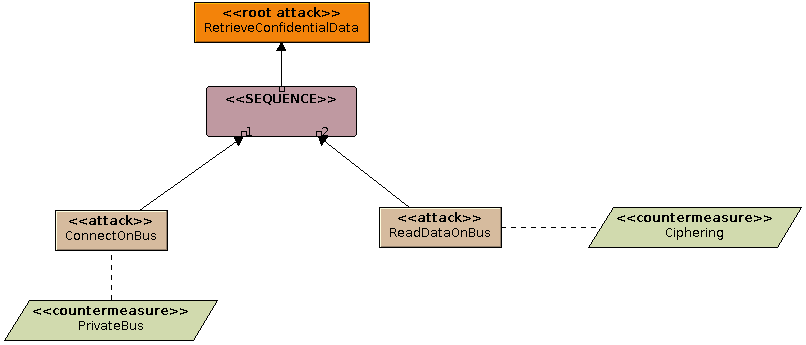
\includegraphics[width=0.8\textwidth]{fig/attacktree.png}
\caption{Attack Tree Model} \label{fig:attacktree}
\end{figure*}

The attack tree of Figure \ref{fig:attacktree} contains a root attack: "RetrieveConfidentialData". This root attack is possible if and only if the attacker first connects to the bus (let's call this attack $att_1$), and then reads (and interprets) a data on the bus ($att_2$). Making either $att_1$ or $att_2$ not possible in our system would be sufficient to ensure that the root attack is not possible. This is obvious in our attack tree, but this is not always the case, such as for larger systems with complex logical combinations of attack steps. Thus, TTool proposes a way to investigate if a given attack is still possible in the system directly from attack trees. Let's try together:
\begin{enumerate}
\item Right click on the root attack, and click on  "Select for Reachability/Liveness".
\item Let's now see if the root attack is reachable. For this, check the syntax of the diagram, and click on the "Safety verification (internal tool)" icon. Then, select "Reachability of selected states" and click on start. Close the window. You diagram should be annotated with a green "R", as shown on Figure \ref{fig:attacktree_verif1}.
\item Let's make $att_1$ or $att_2$ not feasible. For this, you can right click on e.g. $att_1$ and select "Disable". If an attack is disabled, it probably means that a countermeasure has been used. Thus, countermeasure blocks can be linked to attacks. In the case of $ att_1$, the countermeasure is to make the bus private (e.g., make it internal to a chip if the attacker has no way to investigate a bus within a chip). For $att_2$, a common countermeasure is to use security protocols relying on ciphering algorithms. For now, we assume that only $att_1$ is disabled. Run the verification process again. After this verification process, you should obtain a red "R", meaning that the root attack is no longer feasible (see Figure \ref{fig:attacktree_verif2})
 \end{enumerate}


\begin{figure*}[htbp]
\centering
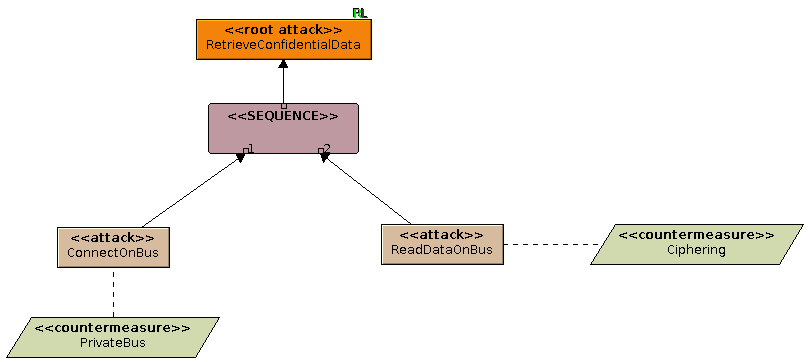
\includegraphics[width=0.8\textwidth]{fig/attacktree_verif1.png}
\caption{Attack Tree Model after formal verification with no attack steps disabled} \label{fig:attacktree_verif1}
\end{figure*}

\begin{figure*}[htbp]
\centering
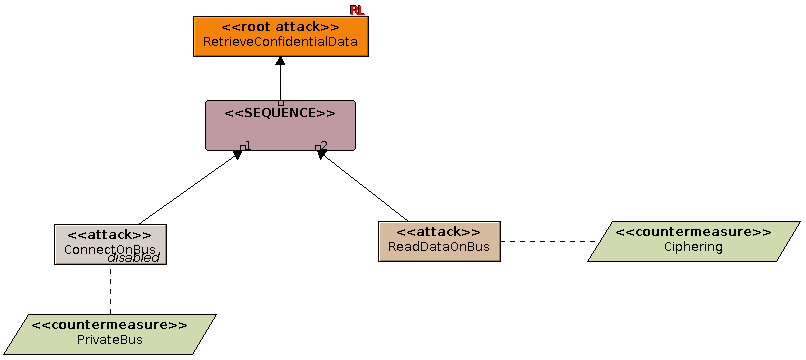
\includegraphics[width=0.8\textwidth]{fig/attacktree_verif2.png}
\caption{Attack Tree Model after formal verification with attack steps disabled by countermeasures} \label{fig:attacktree_verif2}
\end{figure*}

\subsection{Implementing security countermeasures}

\subsubsection{Security verification}
Before implementing security countermeasures in the mapping model, this document explains how to perform formal security
 verification. Again, Figure \ref{fig:fv1} contains a security property on channel "comm" to verify that the latter is confidential. Let's now prove this confidentiality property on the first system version (see Figure \ref{fig:mapping1}):
\begin{enumerate}
\item Check the syntax of "NonSecureArchitectureWithNonSecureFV" diagram.
\item Click on the "SecurityVerification (ProVerif)" icon. A dialog window should open: click on start. The results should be as shown in Figure \ref{fig:proverif1}.
\item The result of the verification is displayed in the lower part of Figure \ref{fig:proverif1}. There are two results:
\begin{itemize}
\item The $comm$ channel is NOT confidential, which proves that the confidentiality requirement is NOT satisfied
\item The read and write actions in T2 and T1 are reachable. This result is important in the case the property is satisfied. Indeed, if none of these actions were reachable, the channel would be confidential since there would be no exchange of data on this channel.
\end{itemize}
\item Since $comm$ is not confidential, TTool can draw an attack trace that shows how the attacker manages to retrieve the data. Right click on the non satisfied authenticity, and select "show trace" (see Figure \ref{fig:trace1}). This (obvious) trace explains that T1 directly send a data to the attacker since T1 writes the data on a public bus.
\item The functional view is annotated with the verification results, as shown on Figure \ref{fig:fv1results}.
\end{enumerate}

\begin{figure*}[htbp]
\centering
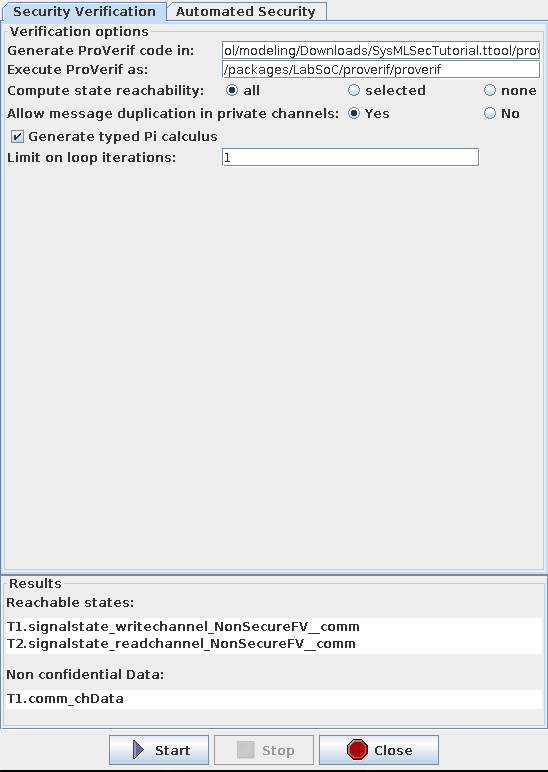
\includegraphics[width=0.6\textwidth]{fig/proverif1.png}
\caption{Security verification dialog window} \label{fig:proverif1}
\end{figure*}


\begin{figure*}[htbp]
\centering
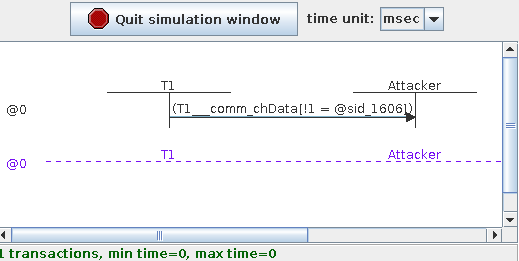
\includegraphics[width=0.6\textwidth]{fig/trace1.png}
\caption{Attack trace} \label{fig:trace1}
\end{figure*}

\begin{figure*}[htbp]
\centering
\includegraphics[width=0.1\textwidth]{build/fv1_t1_results-svg.pdf}
\includegraphics[width=0.7\textwidth]{build/fv1_results-svg.pdf}
\includegraphics[width=0.1\textwidth]{build/fv1_t2_results-svg.pdf}
\caption{Functional View annotated with security verification} \label{fig:fv1results}
\end{figure*}

\subsubsection{Countermeasure 1: Secure Bus}
As seen before, a first countermeasure is to use a secure bus, which is called "private" in TTool. Thus, the bus in the second mapping (called "SecureArchitectureWithNonSecureFV") is private. You can see this with the green shield icon on the bus. A double-click on this bus makes it possible to change this parameter (public, private).

Try to run the security verification of this second system. You should observe that the confidentiality property is now verified.

\begin{figure*}[htbp]
\centering
\includegraphics[width=0.6\textwidth]{build/mapping2-svg}
\caption{Secure Architecture due to a private bus} \label{fig:mapping2}
\end{figure*}

\subsubsection{Countermeasure 2: Secure Functions}
A second countermeasure consists in adding security mechanisms to the two functions T1 and T2. TTool offers cryptographic configurations to add security mechanisms to the behaviour of blocks (See our Modelsward 2017 paper). Basically, a cryptographic configuration specifies the type of security mechanism (symmetric cipher, hash, key manipulation, nonce, etc.) and its performance impact in terms of complexity operations by sample.

The modified activity diagrams of T1 and T2 are given in Figure \ref{fig:fv3}. Note that only the activity diagrams have been modified with regards to previous version.

\begin{figure*}[htbp]
\centering
\includegraphics[width=0.2\textwidth]{build/fv3_t1-svg.pdf}
\includegraphics[width=0.4\textwidth]{build/fv3-svg.pdf}
\includegraphics[width=0.2\textwidth]{build/fv3_t2-svg.pdf}
\caption{Functional view updated with cryptographic configurations} \label{fig:fv3}
\end{figure*}

If you double-click on the SE operator of T1, the following windows should open (see Figure \ref{fig:ccdialog}). This dialog window contains the following fields:
\begin{itemize}
\item \textbf{Name} of the configuration. This name is useful to reference a given cryptographic configuration when writing/reading data. For instance, the write operator on $comm$ in T1 uses the Cipherdata cryptographic configuration.
\item The \textbf{type} of the cryptographic configuration: Symmetric, Asymmetric, MAC, Hash, Nonce, Advanced. In our case, a symmetric encryption is selected.
\item The \textbf{complexity}, in terms of integer operations, of the selected operation
\item The use of \textbf{cryptographic material}: keys, nonces and precise algorithm (AES, etc.) 
\end{itemize}


\begin{figure*}[htbp]
\centering
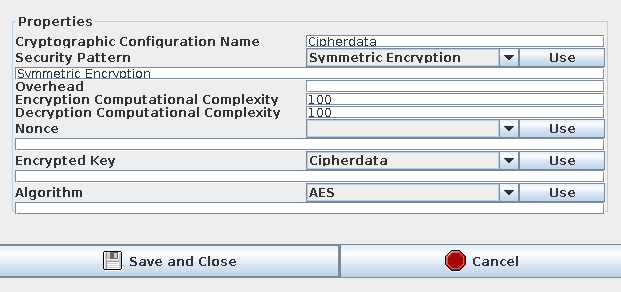
\includegraphics[width=0.7\textwidth]{fig/ccdialog.png}
\caption{Cryptographic configuration dialog window} \label{fig:ccdialog}
\end{figure*}

Let's now consider a third mapping (named "NonSecureArchitectureWithSecureFV") which basically consists in mapping the secure tasks to the non secure architecture (i.e., the one with the public bus). The result of the security verification of this system is given in Figure \ref{fig:fv3_result}. The confidentiality property is now verified.

\begin{figure*}[htbp]
\centering
\includegraphics[width=0.7\textwidth]{build/fv3_result-svg}
\caption{Verification result in the case of a non secure architecture but with secure functions} \label{fig:fv3_result}
\end{figure*}

Unfortunately, security mechanisms impact the performance of the system. TTool makes it possible to evaluate the performance of two different mappings,e.g. the one with no security (version 1), and the one with security mechanisms (version 3). To do this, TTool relies on the DIPLODOCUS simulator\footnote{see the tutorial on DIPLODOCUS to learn how to use the DIPLODOCUS simulator: https://ttool.telecom-paristech.fr/diplodocus.html}.

Without taking into account penalties of the hardware platform (e.g. cache miss, task switching time, boot time, etc.), simulation takes 20 cycles in the case of the non secure system (see Figure \ref{fig:simu_mapping1}), and 220 (20 cycles + 100 cycles for ciphering + 100 cycles for deciphering) in the case of the secure mechanisms added to tasks(see Figure \ref{fig:simu_mapping3}).

\begin{figure*}[htbp]
\centering
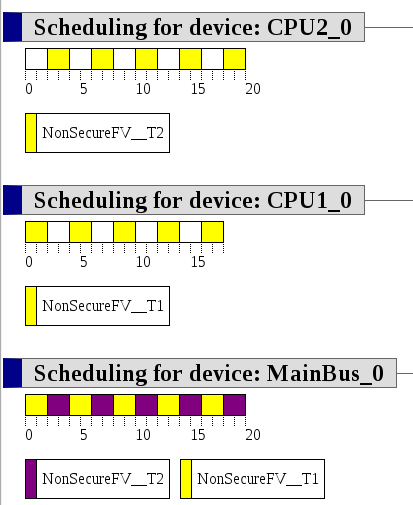
\includegraphics[width=0.5\textwidth]{fig/simu_mapping1}
\caption{Simulation of non secure application mapped on the non secure architecture} \label{fig:simu_mapping1}
\end{figure*}

\begin{figure*}[htbp]
\centering
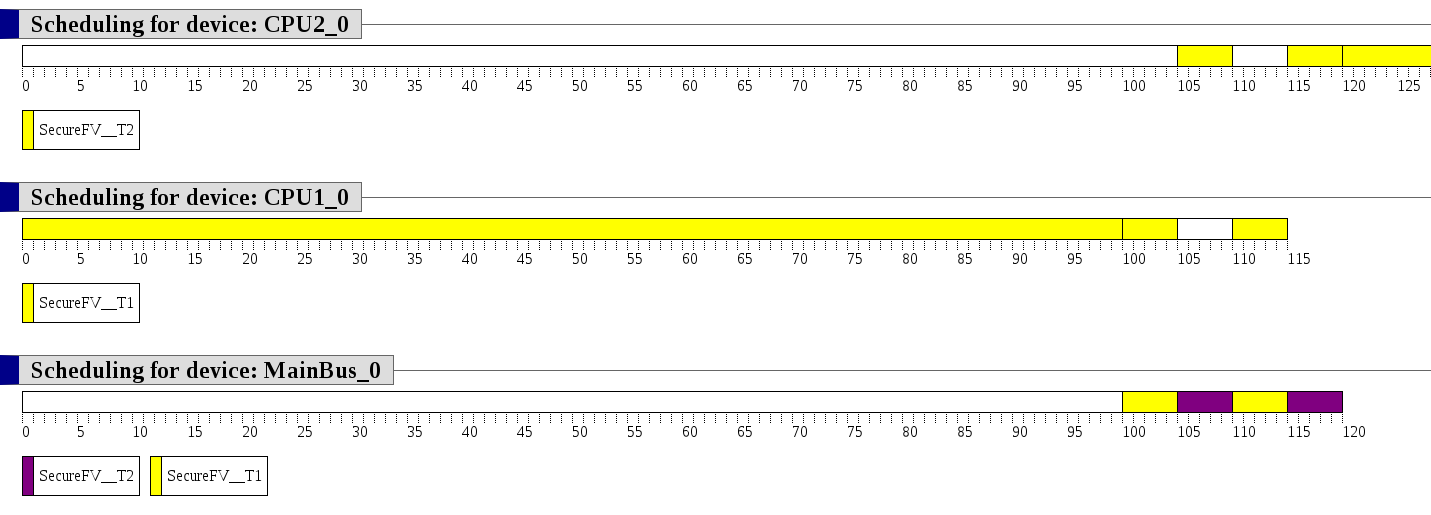
\includegraphics[width=0.99\textwidth]{fig/simu_mapping3}
\caption{Excerpt of the simulation of the secure application mapped on the non secure architecture} \label{fig:simu_mapping3}
\end{figure*}

\subsection{Designing security protocols}
During the HW/SW partitioning stage, security mechanisms have been modeled at a high level of abstraction, mostly to place them correctly in the system, and to evaluate their impact on the system performance. During the software design stage, security protocols can be designed in a more precise way.

A software design contains a block diagram (see Figure \ref{fig:design}) as well as a state machine for each task block (see Figure \ref{fig:design_t}). 

The block diagram contains a main block ("System") with two sub blocks ("T1" and "T2"). These tasks correspond to the same tasks modeled in the HW/SW Partitioning phase at a higher level of abstraction. Two other blocks "Key" and "Messages" are used to define custom data types. T1 and T2 are cryptoblocks, i.e. they define default cryptographic methods e.g. encrypt, decrypt, hash, mac, message manipulation (concat, cut), etc. Last, a pragma:
\begin{itemize}
\item links cryptographic keys of T1 and T2. This key "sk" is system-wide, which means that it is shared once for all protocol sessions.
\item gives a security property to check: the value of the attribute "secretData" of "T1" must remain confidential. 
\end{itemize}


\begin{figure*}[htbp]
\centering
\includegraphics[width=0.9\textwidth]{build/design-svg.pdf}
\caption{Design of a security protocol} \label{fig:design}
\end{figure*}

\begin{figure*}[htbp]
\centering
\includegraphics[width=0.2\textwidth]{build/design_t1-svg.pdf}\hspace{3cm}
\includegraphics[width=0.35\textwidth]{build/design_t2-svg.pdf}
\caption{State machines of T1 (on the left) and T2 (on the right)} \label{fig:design_t}
\end{figure*}

The security formal verification can be performed from these diagrams. Just like for HW/SW partitioning models, both security properties and the reachability of states can be studied, and results are back-traced to the diagrams with e.g. green locks when the property is satisfied (see Figure \ref{fig:design_result}).

\begin{figure*}[htbp]
\centering
\includegraphics[width=0.9\textwidth]{build/design_result-svg.pdf}
\caption{Result of the security verification} \label{fig:design_result}
\end{figure*}


\end{document}
